\documentclass[10pt]{beamer}
 
\usepackage[T1]{fontenc}
\usepackage[utf8]{inputenc}
\usepackage{graphicx}
\usepackage{hyperref}
\usepackage{lmodern}
\usepackage{listings}
\usepackage{amssymb} 
\usepackage{xcolor}
\usetheme{Warsaw}
\usepackage{tikz}
\setbeamercovered{transparent}

\author{Latrille Thibault, Laurent Duret, Nicolas Lartillot}
\title{The red queen dynamic in the kingdom of recombination.}  
\institute{Laboratoire de Biométrie et Biologie Évolutive (LBBE), UMR CNRS 5558, Lyon}

\sloppy 

 
\begin{document}

\frame{\titlepage} 

\begin{frame}
	\begin{center}
       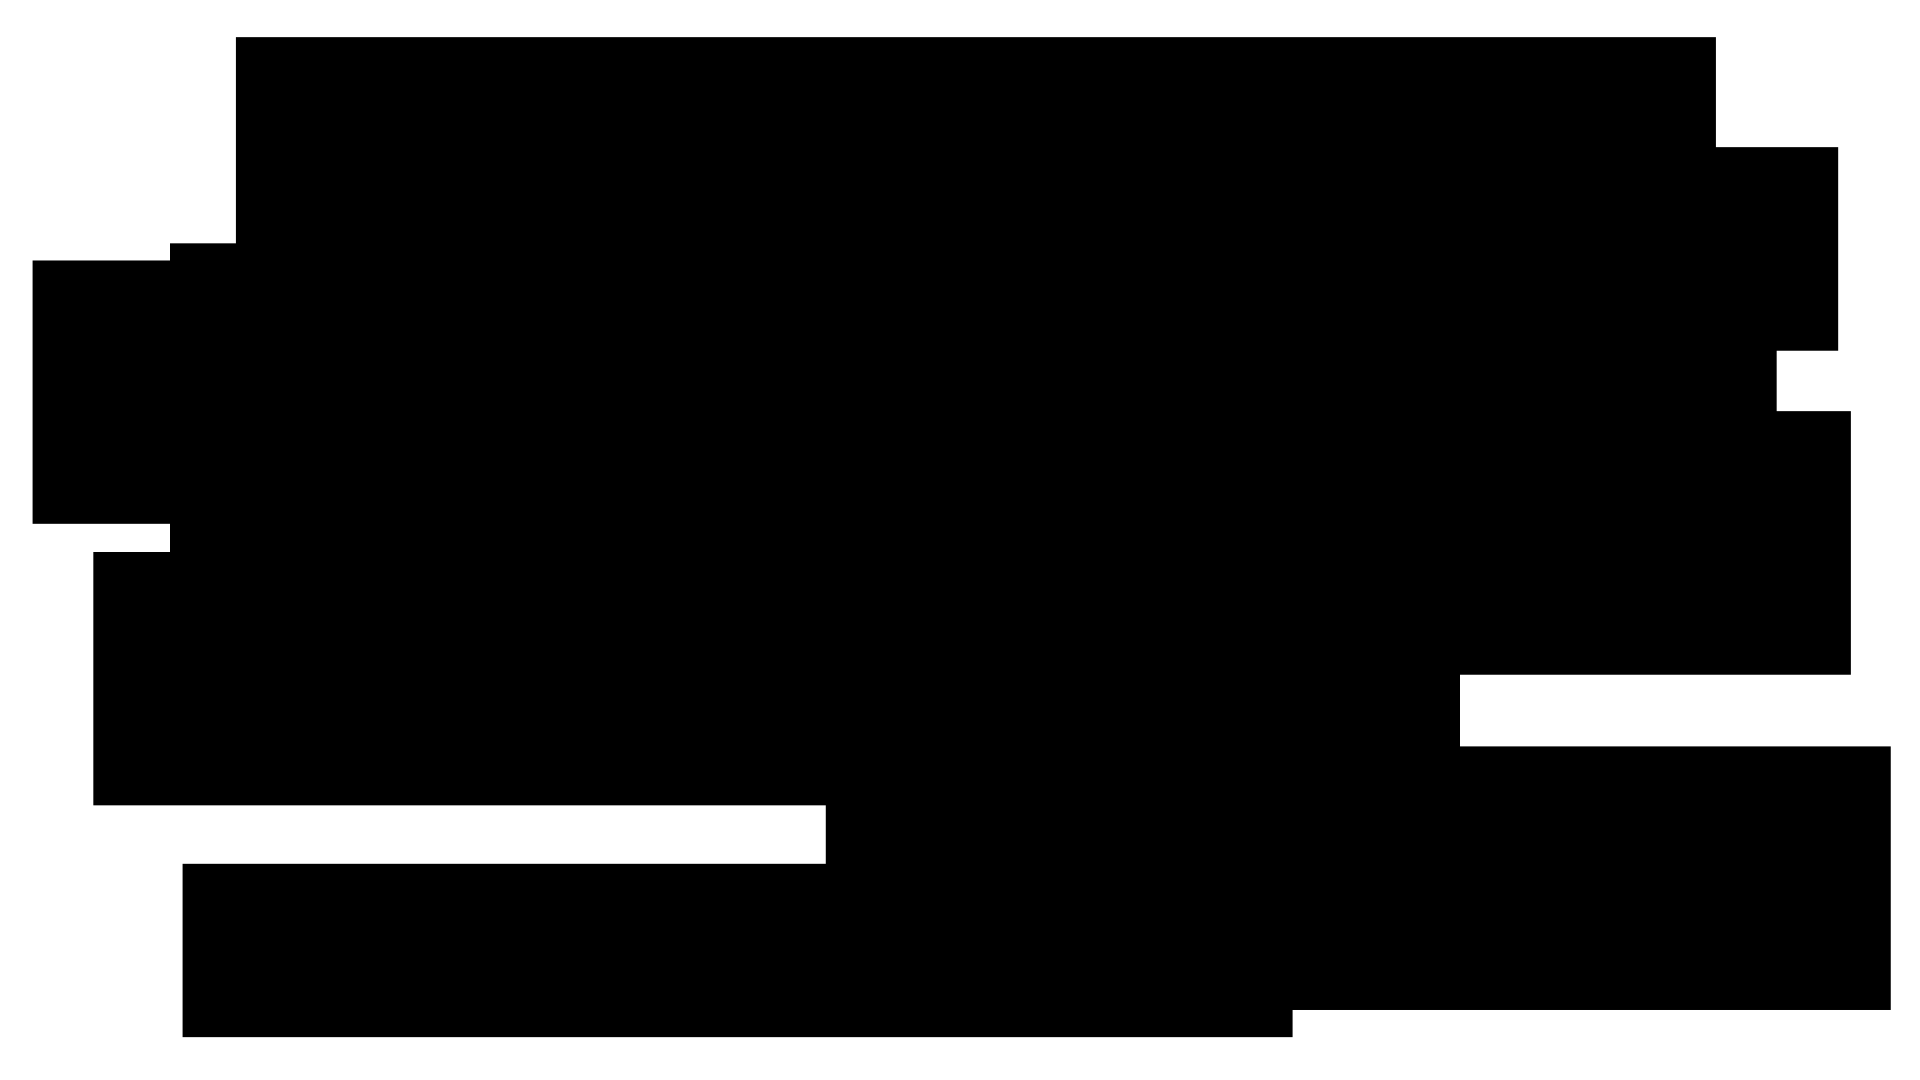
\includegraphics[width=11cm]{Images/publications.png}
	\end{center}
\end{frame}

\begin{frame}
\frametitle{Overline of the presentation}
	\begin{center}
       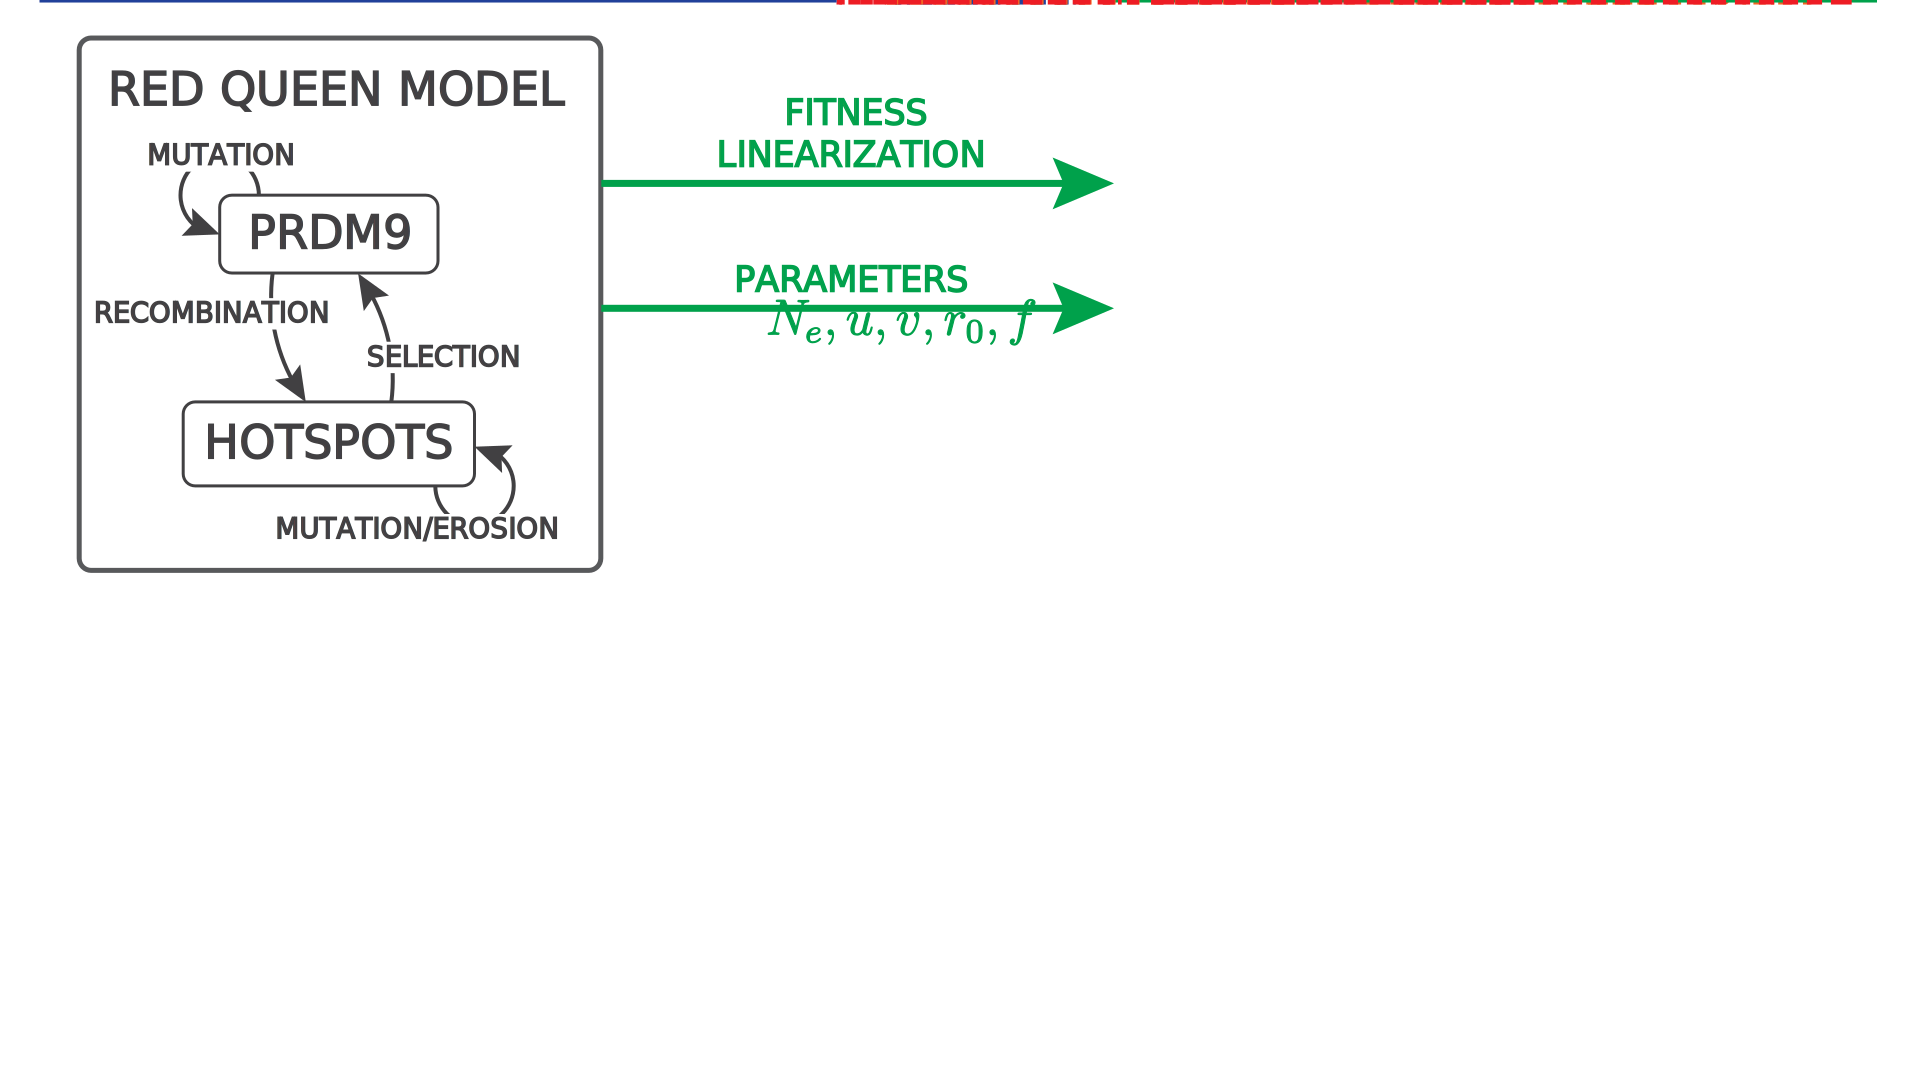
\includegraphics[width=8.5cm]{Images/overline.png}
	\end{center}
\end{frame}

\section{Red queen model}

\begin{frame}
	\begin{center}
	\huge
	Chapter 1. \\
       Red queen model
	\end{center}
\end{frame}

\begin{frame}
	\begin{center}
       \includegraphics[width=8.5cm]{Images/overline-1.png}
	\end{center}
\end{frame}

\begin{frame}
\frametitle{Recombination of the hotspots ruled by PRDM9}
	\begin{center}
       \includegraphics[width=9cm]{Images/red-queen-1.png}
	\end{center}
\end{frame}

\begin{frame}
\frametitle{Erosion of the hotspots and selection of PRDM9}
	\begin{center}
       \includegraphics[width=9cm]{Images/red-queen-2.png}
	\end{center}
\end{frame}

\begin{frame}
\frametitle{Mutation of PRDM9}
	\begin{center}
       \includegraphics[width=9cm]{Images/red-queen-4.png}
	\end{center}
\end{frame}

\begin{frame}
\frametitle{Erosion, again and again...}
	\begin{center}
       \includegraphics[width=9cm]{Images/red-queen-5.png}
	\end{center}
\end{frame}

\section{Population genetic model}

\begin{frame}
	\begin{center}
	\huge
	Chapter 2. \\
       Population genetic model
	\end{center}
\end{frame}

\begin{frame}
	\begin{center}
       \includegraphics[width=8.5cm]{Images/overline-2.png}
	\end{center}
\end{frame}

\begin{frame}
	\frametitle{Parameters}
	\begin{center}
       \includegraphics[width=9cm]{Images/red-queen-model.jpg}
	\end{center}
\end{frame}

\begin{frame}
	\begin{center}
		\Large
    Erosion of the hotspots.
	\end{center}

	$\bullet$ $\forall i \in \{ 1, \, \dots, \, K \} $, $K$ is the number of variants in the population.
		
	$\bullet$ $x_i$ is the frequency of the $i^{th}$ PRDM9 variant.\\
	
	$\bullet$ $l_i$ is the proportion of hot hotspots associated to the $i^{th}$ PRDM9 variant.\\
	
	$\bullet$ $N_e$ is the population size.\\
	
	$\bullet$ $v$ is the mutation rate at the hotspot.\\
	
	$\bullet$ $r_0$ is the recombination rate.\\
		\begin{enumerate}
	\item Substitution from hot to cold at a rate $ 2 N_e v  l_i $ \\
	\item Selection at a rate $2 r_0 x_i $
	\end{enumerate}
\[
      \begin{aligned}
        \dfrac{\mathrm{d}l_i}{\mathrm{d}t} &= 
        - 4 N_e v r_0 x_i l_i \\
      \end{aligned}
\]
\end{frame}

\begin{frame}
	\begin{center}
		\Large
    Mutation and selection of PRDM9.
	\end{center}

		$\bullet$ $\forall i \in \{ 1, \, \dots, \, K \} $, $K$ is the number of variants in the population.
		
	$\bullet$ $x_i$ is the frequency of the $i^{th}$ PRDM9 variant.\\
	
	$\bullet$ $l_i$ is the proportion of hot hotspots associated to the $i^{th}$ PRDM9 variant.\\
	
	$\bullet$ $N_e$ is the population size.\\
	
	$\bullet$ $u$ is the mutation rate of PRDM9.\\

	$\bullet$ $\overline{\omega_i}=\sum_j x_j f \left( \tfrac{L_i + L_j}{2} \right)$ is the fitness of the $i^{th}$ PRDM9 variant.\\
	
	$\bullet$ $\overline{\omega}=\sum_{i} x_i \overline{\omega_i}$ is the mean fitness in the population.\\
		\begin{enumerate}
	\item New variant from a Poisson distribution at a rate $ 2 N_e u $ per generation. \\
	\item The probability of drawing variant $i$ in the new generation is $ \tfrac{x_i \overline{\omega_i}}{\overline{\omega}} $
		\end{enumerate}
\end{frame}

\begin{frame}
	\frametitle{Parameters}
	\begin{center}
       \includegraphics[width=9cm]{Images/red-queen-model.jpg}
	\end{center}
\end{frame}

\begin{frame}
	\frametitle{Trajectory}
	\begin{center}
       \includegraphics[width=10.5cm]{Images/simulations.png}
	\end{center}
\end{frame}

\section{Results}

\begin{frame}
	\begin{center}
	\huge
	Chapter 3. \\
       Results
	\end{center}
\end{frame}


\begin{frame}
\frametitle{Results}
	\begin{center}
       \includegraphics[width=8.5cm]{Images/overline-3.png}
	\end{center}
\end{frame}

\begin{frame}
	\begin{center}
		\Large
    	Definition of the PRDM9's diversity $K_e$ 
    \end{center}
	Let $x_i$ be the frequency of the $i^{th}$ PRDM9 variant.\\

    \[ K_e = \dfrac{1}{\displaystyle \sum_i x_i^2}   \]
	\begin{center}
       \includegraphics[width=7cm]{Images/ne-diversity.png}
	\end{center}
\end{frame}

\begin{frame}
	\begin{center}
		\begin{enumerate}
		\item $K_e \nearrow$ with the mutation rate of PRDM9 ($u$).
		
		\item $K_e \rightsquigarrow$ with the mutation rate at the hotspots ($v$).
		\end{enumerate}
       \includegraphics[width=11cm]{Images/simpson-entropy-mutation-erosion.png}
	\end{center}
\end{frame}

\begin{frame}
	\begin{center}
		\begin{enumerate}
		\item $K_e \nearrow$ with the the population size ($N_e$).
		
		\item $K_e \nearrow$ with the mutation rate of PRDM9 ($u$).
		\end{enumerate}
       \includegraphics[width=11cm]{Images/simpson-entropy-population-mutation.png}
	\end{center}
\end{frame}

\begin{frame}
	\begin{center}
		\begin{enumerate}
		\item $K_e \nearrow$ with the the population size ($N_e$).
		
		\item $K_e \rightsquigarrow$ with the mutation rate at the hotspots ($v$).
		\end{enumerate}
       \includegraphics[width=11cm]{Images/simpson-entropy-population-erosion.png}
	\end{center}
\end{frame}


\begin{frame}
	\begin{center}
		\Large
    	Evolution of the PRDM9's diversity $K_e$ 
	\end{center}
	$ N_e $ is the population size. \\ 
	$ u $ is the mutation rate of PRDM9. \\
	\begin{enumerate}
		\item $ N_e u \ll 1 \Rightarrow  K_e \simeq 1$ (single allele succession)
		\item $ N_e u \gg 1 \Rightarrow  K_e > 1 $ (polymorphism)
		
		\item $K_e \nearrow$ with $N_e$ and $u$.
		
		\item $K_e \rightsquigarrow$ with the mutation ($v$) and recombination rate at the hotspots ($r_o$)
		
		\item $K_e \rightsquigarrow$ with the fitness function.
	\end{enumerate}
\end{frame}


\begin{frame}
	\begin{center}
		\Large
    	Definition of the mean fraction of hot hotspots $\bar{L}$ 
    \end{center}
	Let $x_i$ be the frequency of the $i^{th}$ PRDM9 variant.\\
	Let $l_i$ be the fraction of hot hotspots (still not eroded) associated with the $i^{th}$ PRDM9 variant.\\

    \[ \bar{L} =  \sum_i x_i l_i   \]
	\begin{center}
       \includegraphics[width=7cm]{Images/ne-mean-erosion.png}
	\end{center}
\end{frame}

\begin{frame}
	\begin{center}
		\begin{enumerate}
		\item $\bar{L} \nearrow$ with the mutation rate of PRDM9 ($u$).
		
		\item $\bar{L} \searrow$ with the mutation rate at the hotspots ($v$).
	\end{enumerate}
       \includegraphics[width=11cm]{Images/mean-erosion-mutation-erosion.png}
	\end{center}
\end{frame}

\begin{frame}
	\begin{center}
		\begin{enumerate}
		\item $\bar{L} \rightsquigarrow$ with the population size ($N_e$).
		
		\item $\bar{L} \nearrow$ with the mutation rate of PRDM9 ($u$).
	\end{enumerate}
       \includegraphics[width=11cm]{Images/mean-erosion-population-mutation.png}
	\end{center}
\end{frame}

\begin{frame}
	\begin{center}
		\begin{enumerate}
		\item $\bar{L} \rightsquigarrow$ with the population size ($N_e$).
				
		\item $\bar{L} \nearrow$ with the mutation rate at the hotspots ($v$).
	\end{enumerate}
       \includegraphics[width=11cm]{Images/mean-erosion-population-erosion.png}
	\end{center}
\end{frame}


\begin{frame}
	\begin{center}
		\Large
    	Evolution of the mean fraction of hot hotspots $\bar{L}$
	\end{center}
	\begin{enumerate}
			
		\item $\bar{L} \rightsquigarrow$ with the population size ($N_e$).
				
		\item $\bar{L} \nearrow$ with the mutation rate of PRDM9. ($u$).
		
		\item $\bar{L} \searrow$ with the mutation ($v$) and recombination rate at the hotspots ($r_o$).

		\item 	The fitness function can be linearised around the mean erosion $\bar{L}$.
	\end{enumerate}
\end{frame}

\begin{frame}
	\begin{center}
		\Large
    	Definition of the turn-over rate $\tau$ 
    \end{center}
	$\tau$ is the number of generations needed to replace all PRDM9 variants. \\
	It is such that the homozygosity between $x_i(t)$ and $x_i(t+\tau)$ vanishes.
	\begin{center}
       \includegraphics[width=7cm]{Images/ne-turn-over.png}
	\end{center}
\end{frame}

\begin{frame}
	\begin{center}
		\begin{enumerate}
		\item $\tau \searrow$ and $\nearrow$ with the mutation rate of PRDM9 ($u$).
		
		\item $\tau \searrow$ with the mutation rate at the hotspots ($v$).
		\end{enumerate}
       \includegraphics[width=11cm]{Images/cross-homozygosity-mutation-erosion.png}
	\end{center}
\end{frame}

\begin{frame}
	\begin{center}
		\begin{enumerate}
		\item $\tau \searrow$ and $\rightsquigarrow$ with the population size ($N_e$).
			
		\item $\tau \searrow$ with the mutation rate of PRDM9 ($u$).
		\end{enumerate}
       \includegraphics[width=11cm]{Images/cross-homozygosity-population-mutation.png}
	\end{center}
\end{frame}

\begin{frame}
	\begin{center}
		\begin{enumerate}
		\item $\tau \searrow$ and $\rightsquigarrow$ with the population size ($N_e$).
			
		\item $\tau \searrow$ with the mutation rate at the hotspots ($v$).
		\end{enumerate}
       \includegraphics[width=11cm]{Images/cross-homozygosity-population-erosion.png}
	\end{center}
\end{frame}

\begin{frame}
	\begin{center}
		\Large
    	Evolution of the turn-over rate $\tau$
	\end{center}
	\begin{enumerate}
		\item $\tau \searrow$ and $\rightsquigarrow$ with the population size ($N_e$).
			
		\item $\tau \searrow$ and $\nearrow$ with the mutation rate of PRDM9. ($u$).
		
		\item $\tau \searrow$ with the mutation ($v$) and recombination rate at the hotspots ($r_o$).
	\end{enumerate}
\end{frame}

\begin{frame}
	\begin{center}
		\Large
		Summary of results
       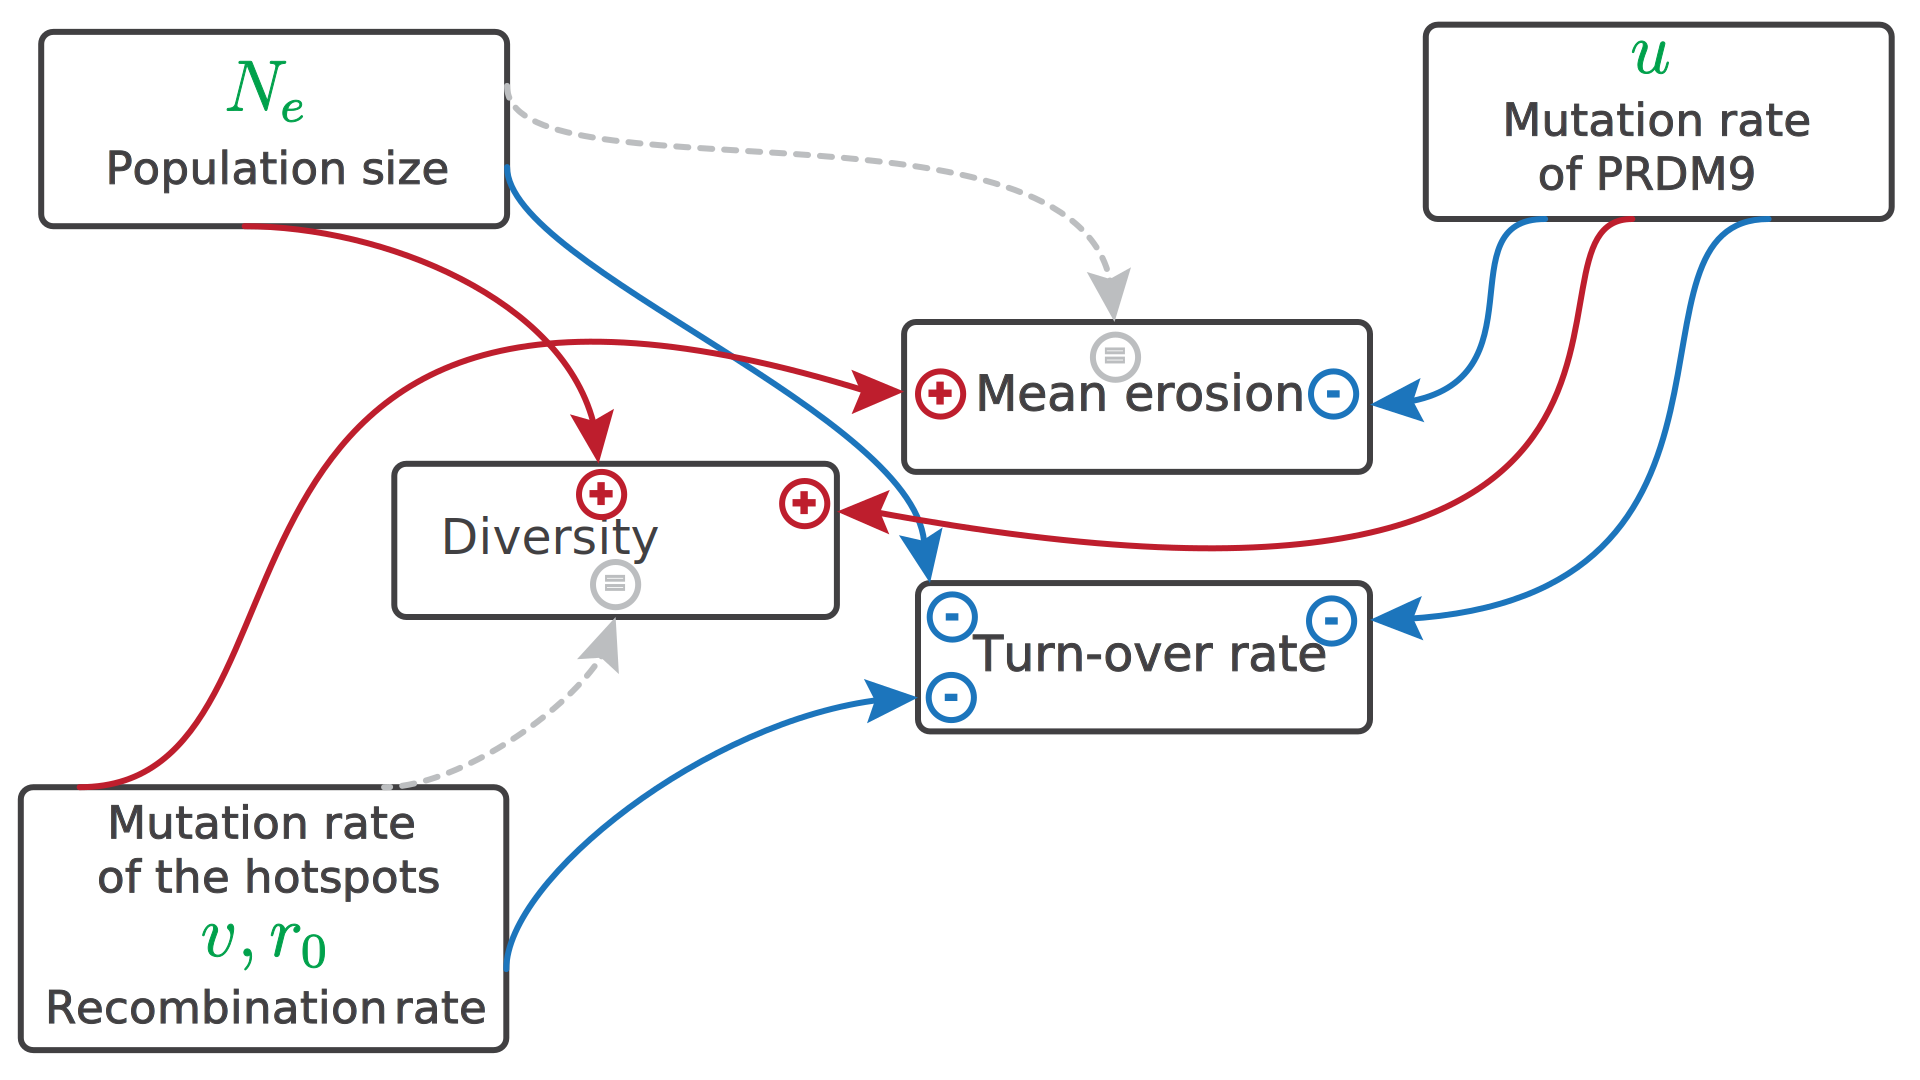
\includegraphics[width=11cm]{Images/summary.png}
	\end{center}
\end{frame}

\section{Single allele equations}

\begin{frame}
	\begin{center}
	\huge
	Chapter 4. \\
       Single allele equations
	\end{center}
\end{frame}

\begin{frame}
\frametitle{Single allele equations}
	\begin{center}
       \includegraphics[width=8.5cm]{Images/overline-4.png}
	\end{center}
\end{frame}

\begin{frame}
	\begin{center}
		\Large
    	Equation for all variants in the population.
	\end{center}
	\begin{enumerate}
	\item $\forall i \in \{ 1, \, \dots, \, K \} $, $K$ is the number of variants in the population.
		
	\item $x_i$ is the frequency of the $i^{th}$ PRDM9 variant.\\
	
	\item $l_i$ is the proportion of hot hotspots associated to the $i^{th}$ PRDM9 variant.\\
		
	\item Assume there is no drift. 
	
	\item Linearise the fitness function around the mean erosion $\bar{L} = \sum_i l_i x_i$.
	\end{enumerate}
\[
  \left\{
      \begin{aligned}
          \dfrac{\mathrm{d}x_i}{\mathrm{d}t} &= \dfrac{f'(\overline{L})}{2 f(\overline{L})} \left( l_i - \overline{L} \right) x_i \\
        \dfrac{\mathrm{d}l_i}{\mathrm{d}t} &= 
        - \rho x_i l_i \\
      \end{aligned}
    \right.
\]
\end{frame}

\begin{frame}
	\begin{center}
		\Large
    	Equation for a single variant.
	\end{center}
	\begin{enumerate}
		\item Also, assume $ u N_e \gg 1$, thus $\bar{L}$ is considered fixed and an external parameter.
	\end{enumerate}
	\begin{center}
       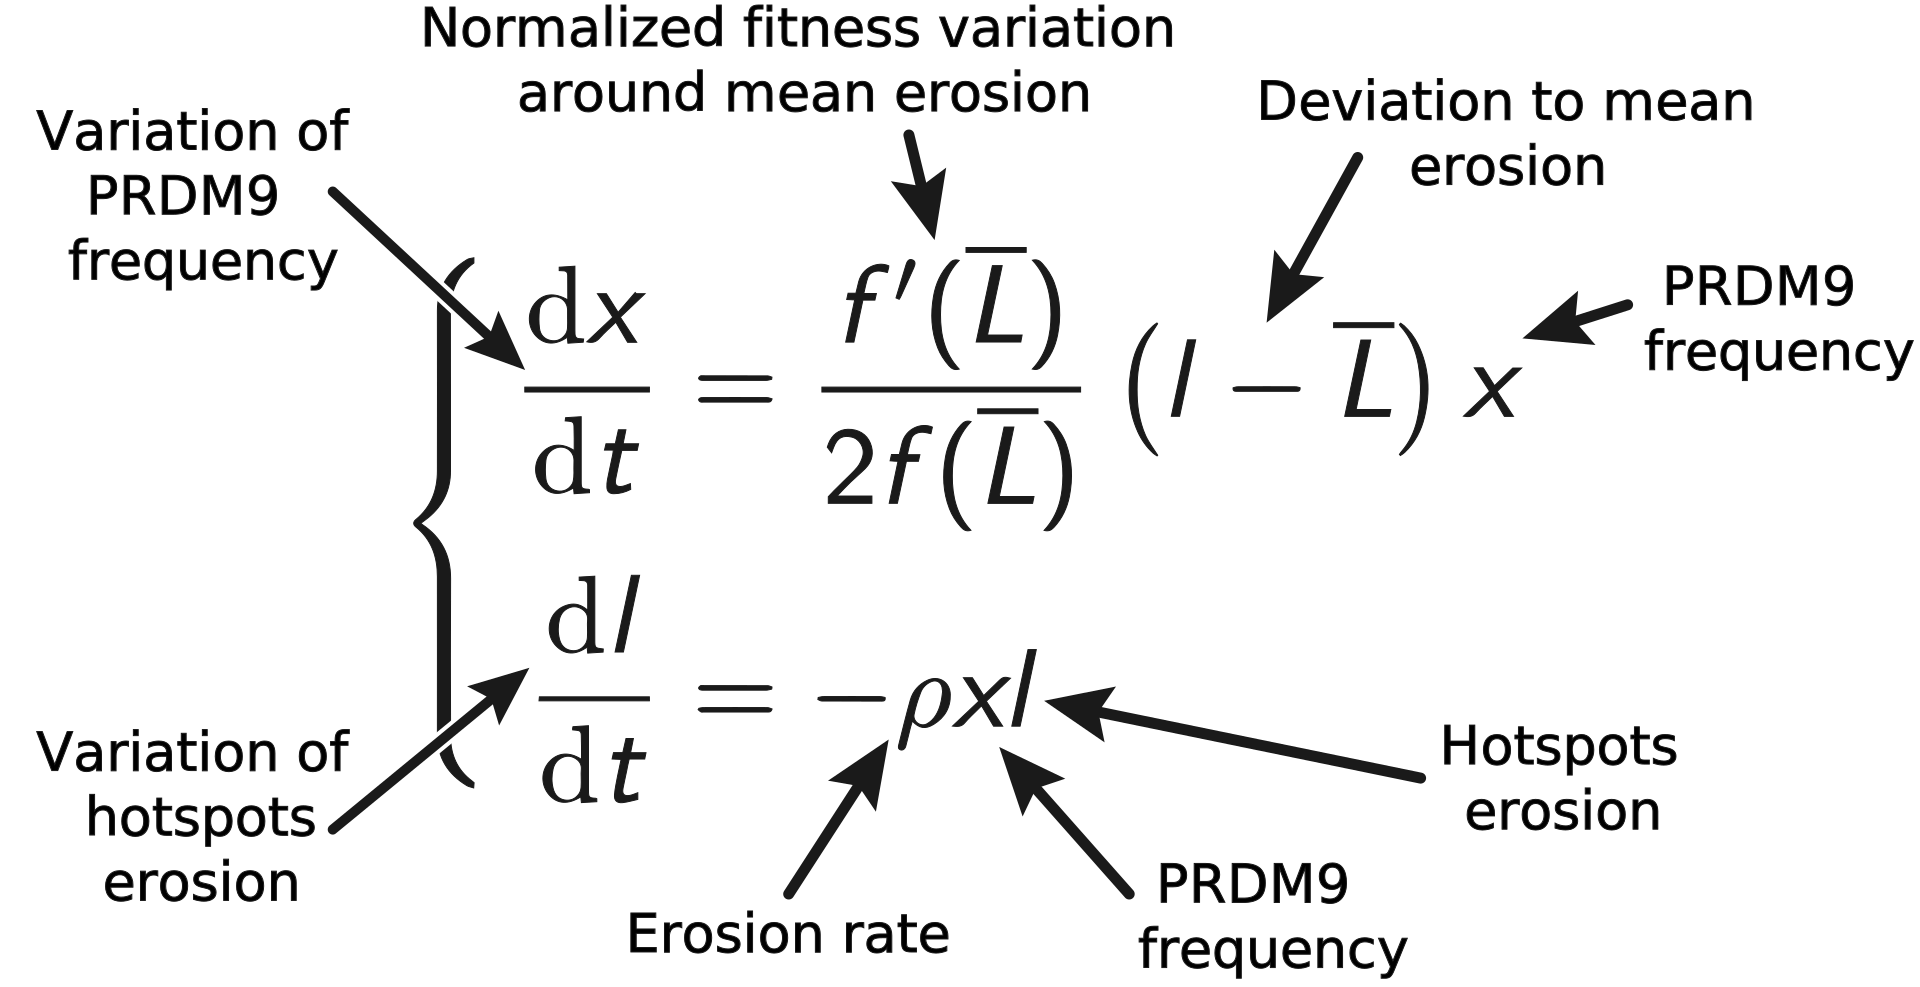
\includegraphics[width=7.5cm]{Images/equation.png}
	\end{center}
\end{frame}

\begin{frame}
\frametitle{Single allele equations}
	\begin{center}
       \includegraphics[width=8cm]{Images/single-allele-differential.png}
	\end{center}
\end{frame}

\begin{frame}
	\begin{center}
		\Large
    	fraction of hot hotspots as an internal clock.
	\end{center}
\[
  \left\{
      \begin{aligned}
          x(l) &=\dfrac{f'(\overline{L})}{2 \rho f(\overline{L})} (1-l + \overline{L} \mathrm{log}(l)) + x_{\mathrm{initial}} \\
           x(l_{\infty}) & \simeq  1-l_{\infty} + \overline{L} \mathrm{log}(l_{\infty}) = 0  \\
      \end{aligned}
    \right.
\]
		$\bullet$ $\rho$ is the scaled erosion rate ($u N_e r_0$). \\
		$\bullet$ $\bar{L}$ is the mean erosion. \\
		$\bullet$ $f$ is the fitness function. \\
\end{frame}

\begin{frame}
\frametitle{Single allele equations}
	\begin{center}
       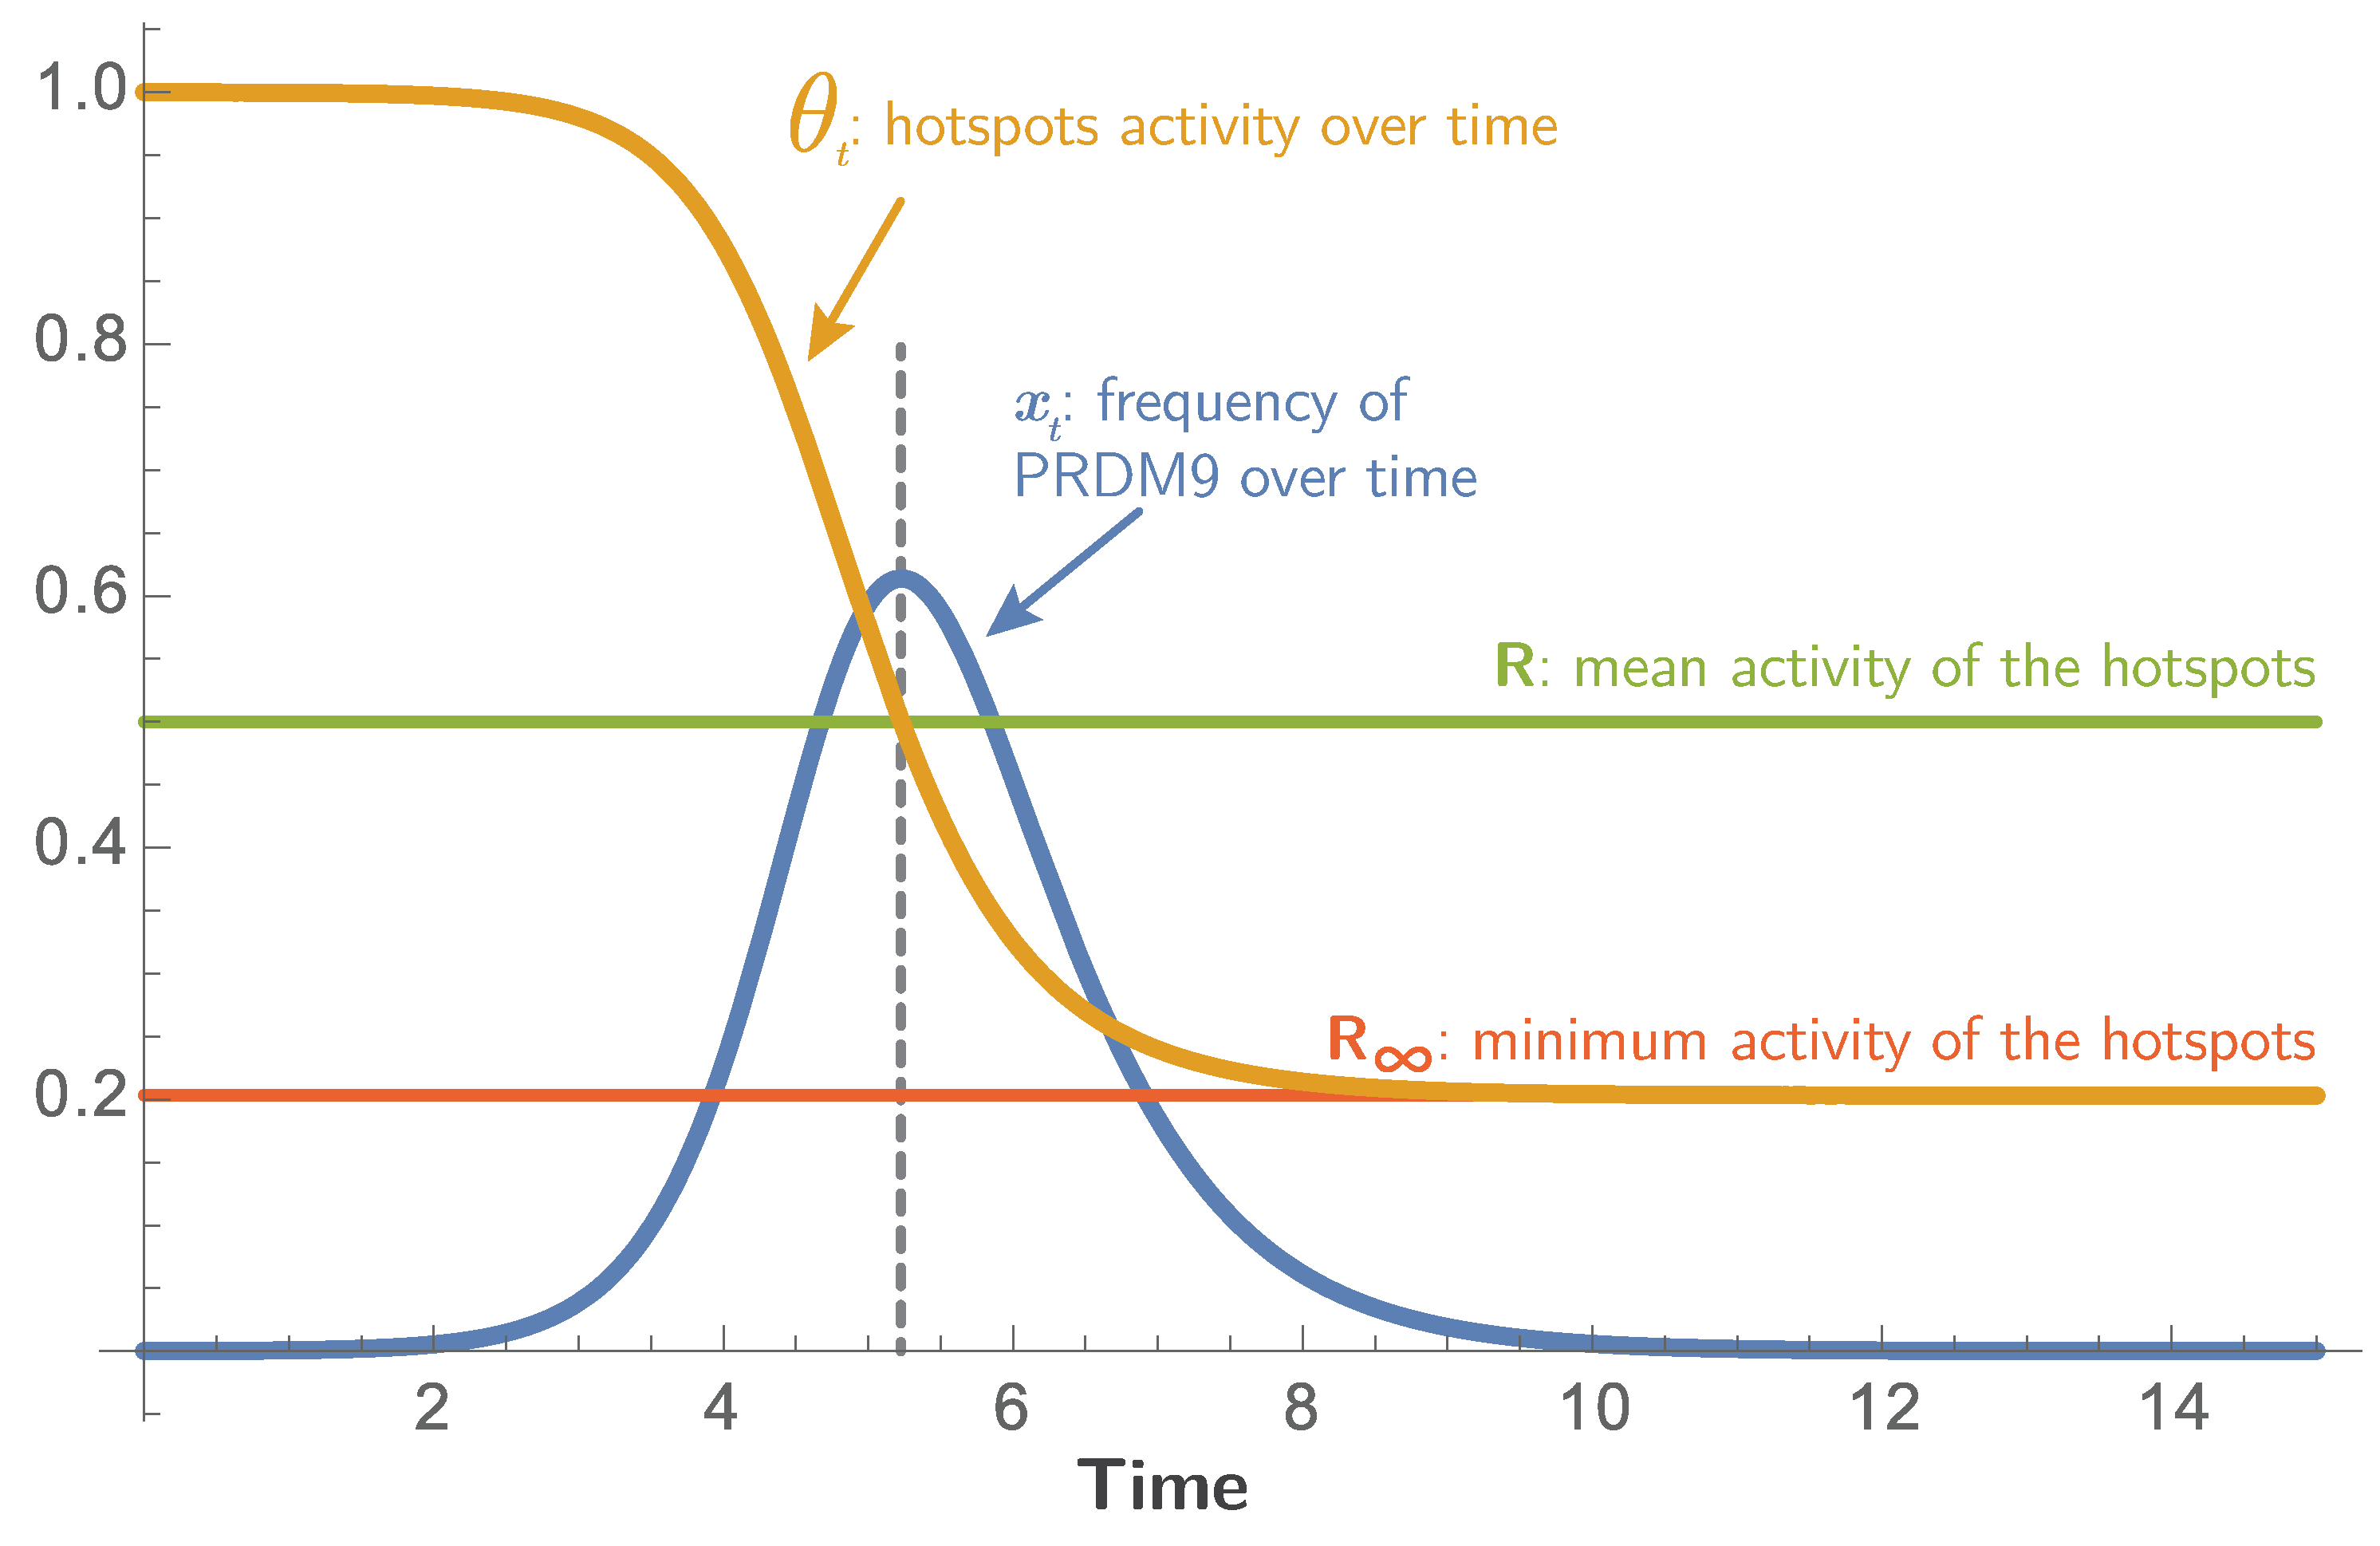
\includegraphics[width=8cm]{Images/single-allele.png}
	\end{center}
\end{frame}

\begin{frame}
	\frametitle{Comparison to simulations}
	\begin{center}
       \includegraphics[width=9cm]{Images/results.png}
	\end{center}
\end{frame}

\begin{frame}
\frametitle{Single allele equations}
	\begin{center}
       \includegraphics[width=8.5cm]{Images/overline-5.png}
	\end{center}
\end{frame}

\begin{frame}
	\begin{center}
		\Large
    Diversity from single allele equations.
	\end{center}
\[
  K_e(\bar{L}) \simeq 
  \dfrac{4 \rho f(\overline{L})}{f'(\overline{L})\left[ 1 + l_{\infty} - 2 \overline{L}  \right]}
\]
	\begin{center}
       \includegraphics[width=11cm]{Images/approximated-diversity.png}
	\end{center}
\end{frame}

\begin{frame}
	\begin{center}
		\Large
    Turn-over rate from single allele equations.
	\end{center}
\[
  \tau (\bar{L}) \sim \dfrac{2 f'(\overline{L})}{f(\overline{L})[\overline{L}-1 + \overline{L} \mathrm{log}(\overline{L})]}
\]
	\begin{center}
       \includegraphics[width=11cm]{Images/approximated-turn-over.png}
	\end{center}
\end{frame}

\begin{frame}
	\begin{center}
		\Large
    Mean erosion estimate.
	\end{center}
\[
  0 \simeq N_e u \dfrac{f(\overline{L})}{2f'(\overline{L})} (1 - \bar{L}) -
  4 N_e v r_o
\]
	\begin{center}
       \includegraphics[width=11cm]{Images/estimated-mean-erosion.png}
	\end{center}
\end{frame}

\begin{frame}
	\begin{center}
		\Large
    Diversity using a plug-in estimate for $\bar{L}$.
	\end{center}
\[
  K_e(\bar{L}) \simeq 
  \dfrac{4 \rho f(\overline{L})}{f'(\overline{L})\left[ 1 + l_{\infty} - 2 \overline{L}  \right]}
\]
	\begin{center}
       \includegraphics[width=11cm]{Images/estimated-diversity.png}
	\end{center}
\end{frame}

\begin{frame}
	\begin{center}
		\Large
    Turn-over rate using a plug-in estimate for $\bar{L}$.
	\end{center}
\[
  \tau (\bar{L}) \sim \dfrac{2 f'(\overline{L})}{f(\overline{L})[\overline{L}-1 + \overline{L} \mathrm{log}(\overline{L})]}
\]
	\begin{center}
       \includegraphics[width=11cm]{Images/estimated-turn-over.png}
	\end{center}
\end{frame}

\end{document}


